\documentclass[12pt]{article}
\usepackage{tikz}
\usetikzlibrary{shapes,arrows,chains,positioning,calc,fit,backgrounds}
\usepackage{graphicx}
\usepackage{float}
\usepackage[a4paper, margin=1.5cm]{geometry}

\begin{document}

\title{Architecture Microservices de DeepSeek et proposition d'une architecture microservices parallèle et multi-middleware}
\maketitle

\section{Architecture Microservices Initiale de DeepSeek}

\begin{figure}[H]
\centering
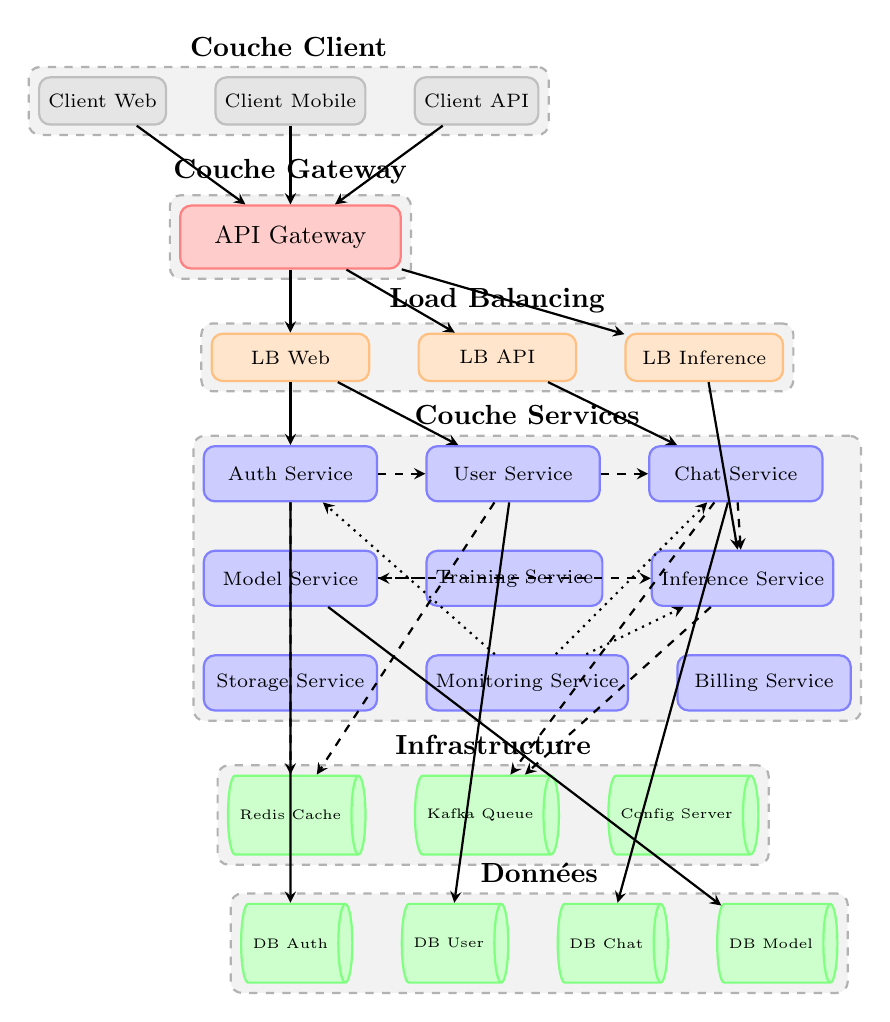
\begin{tikzpicture}[
    node distance=0.8cm and 0.6cm,
    service/.style={rectangle, draw=blue!50, fill=blue!20, thick, minimum width=2.2cm, minimum height=0.7cm, text centered, rounded corners, font=\scriptsize},
    database/.style={cylinder, draw=green!50, fill=green!20, thick, aspect=0.5, minimum height=0.8cm, minimum width=1cm, font=\tiny},
    gateway/.style={rectangle, draw=red!50, fill=red!20, thick, minimum width=2.8cm, minimum height=0.8cm, rounded corners, font=\small},
    loadbalancer/.style={rectangle, draw=orange!50, fill=orange!20, thick, minimum width=2cm, minimum height=0.6cm, rounded corners, font=\scriptsize},
    middleware/.style={rectangle, draw=teal!50, fill=teal!20, thick, minimum width=2cm, minimum height=0.6cm, rounded corners, font=\scriptsize},
    client/.style={rectangle, draw=gray!50, fill=gray!20, thick, minimum width=1.5cm, minimum height=0.6cm, rounded corners, font=\scriptsize},
    layer/.style={rectangle, draw=black!30, dashed, thick, fill=black!5, rounded corners},
    arrow/.style={->, >=stealth, thick}
]

% ============ COUCHE CLIENT ============
\node[client] (web-client) {Client Web};
\node[client, right=of web-client] (mobile-client) {Client Mobile};
\node[client, right=of mobile-client] (api-client) {Client API};

\begin{scope}[on background layer]
\node[layer, fit=(web-client)(mobile-client)(api-client), label=above:\textbf{Couche Client}] (client-layer) {};
\end{scope}

% ============ COUCHE GATEWAY ============
\node[gateway, below=1cm of mobile-client] (api-gateway) {API Gateway};

\begin{scope}[on background layer]
\node[layer, fit=(api-gateway), label=above:\textbf{Couche Gateway}] (gateway-layer) {};
\end{scope}

% ============ COUCHE LOAD BALANCING ============
\node[loadbalancer, below=0.8cm of api-gateway] (lb-web) {LB Web};
\node[loadbalancer, right=of lb-web] (lb-api) {LB API};
\node[loadbalancer, right=of lb-api] (lb-inference) {LB Inference};

\begin{scope}[on background layer]
\node[layer, fit=(lb-web)(lb-api)(lb-inference), label=above:\textbf{Load Balancing}] (lb-layer) {};
\end{scope}

% ============ COUCHE SERVICES ============
\node[service, below=0.8cm of lb-web] (auth-service) {Auth Service};
\node[service, right=of auth-service] (user-service) {User Service};
\node[service, right=of user-service] (chat-service) {Chat Service};

\node[service, below=0.6cm of auth-service] (model-service) {Model Service};
\node[service, right=of model-service] (training-service) {Training Service};
\node[service, right=of training-service] (inference-service) {Inference Service};

% Services support
\node[service, below=0.6cm of model-service] (storage-service) {Storage Service};
\node[service, right=of storage-service] (monitoring-service) {Monitoring Service};
\node[service, right=of monitoring-service] (billing-service) {Billing Service};

\begin{scope}[on background layer]
\node[layer, fit=(auth-service)(user-service)(chat-service)(model-service)(training-service)(inference-service)(storage-service)(monitoring-service)(billing-service), 
      label=above:\textbf{Couche Services}] (services-layer) {};
\end{scope}

% ============ COUCHE INFRASTRUCTURE ============
\node[database, below=0.8cm of storage-service] (cache) {Redis Cache};
\node[database, right=of cache] (mq) {Kafka Queue};
\node[database, right=of mq] (config) {Config Server};

\begin{scope}[on background layer]
\node[layer, fit=(cache)(mq)(config), label=above:\textbf{Infrastructure}] (infra-layer) {};
\end{scope}

% ============ COUCHE DONNÉES ============
\node[database, below=0.6cm of cache] (db-auth) {DB Auth};
\node[database, right=of db-auth] (db-user) {DB User};
\node[database, right=of db-user] (db-chat) {DB Chat};
\node[database, right=of db-chat] (db-model) {DB Model};

\begin{scope}[on background layer]
\node[layer, fit=(db-auth)(db-user)(db-chat)(db-model), label=above:\textbf{Données}] (data-layer) {};
\end{scope}

% ============ CONNEXIONS ============
% Client -> Gateway
\draw[arrow] (web-client) -- (api-gateway);
\draw[arrow] (mobile-client) -- (api-gateway);
\draw[arrow] (api-client) -- (api-gateway);

% Gateway -> Load Balancing
\draw[arrow] (api-gateway) -- (lb-web);
\draw[arrow] (api-gateway) -- (lb-api);
\draw[arrow] (api-gateway) -- (lb-inference);

% Load Balancing -> Services
\draw[arrow] (lb-web) -- (auth-service);
\draw[arrow] (lb-web) -- (user-service);
\draw[arrow] (lb-api) -- (chat-service);
\draw[arrow] (lb-inference) -- (inference-service);

% Communication entre services
\draw[arrow, dashed] (auth-service) -- (user-service);
\draw[arrow, dashed] (user-service) -- (chat-service);
\draw[arrow, dashed] (chat-service) -- (inference-service);
\draw[arrow, dashed] (model-service) -- (inference-service);
\draw[arrow, dashed] (training-service) -- (model-service);

% Services -> Infrastructure
\draw[arrow, dashed] (auth-service) -- (cache);
\draw[arrow, dashed] (user-service) -- (cache);
\draw[arrow, dashed] (chat-service) -- (mq);
\draw[arrow, dashed] (inference-service) -- (mq);

% Services -> Databases
\draw[arrow] (auth-service) -- (db-auth);
\draw[arrow] (user-service) -- (db-user);
\draw[arrow] (chat-service) -- (db-chat);
\draw[arrow] (model-service) -- (db-model);

% Monitoring connections
\draw[arrow, dotted] (monitoring-service) -- (auth-service);
\draw[arrow, dotted] (monitoring-service) -- (chat-service);
\draw[arrow, dotted] (monitoring-service) -- (inference-service);

\end{tikzpicture}
\caption{Architecture Microservices Initiale de DeepSeek}
\label{fig:initial-architecture}
\end{figure}

\section{Architecture Microservices avec Solution Parallèle et Multi-Middleware}

\begin{figure}[H]
\centering
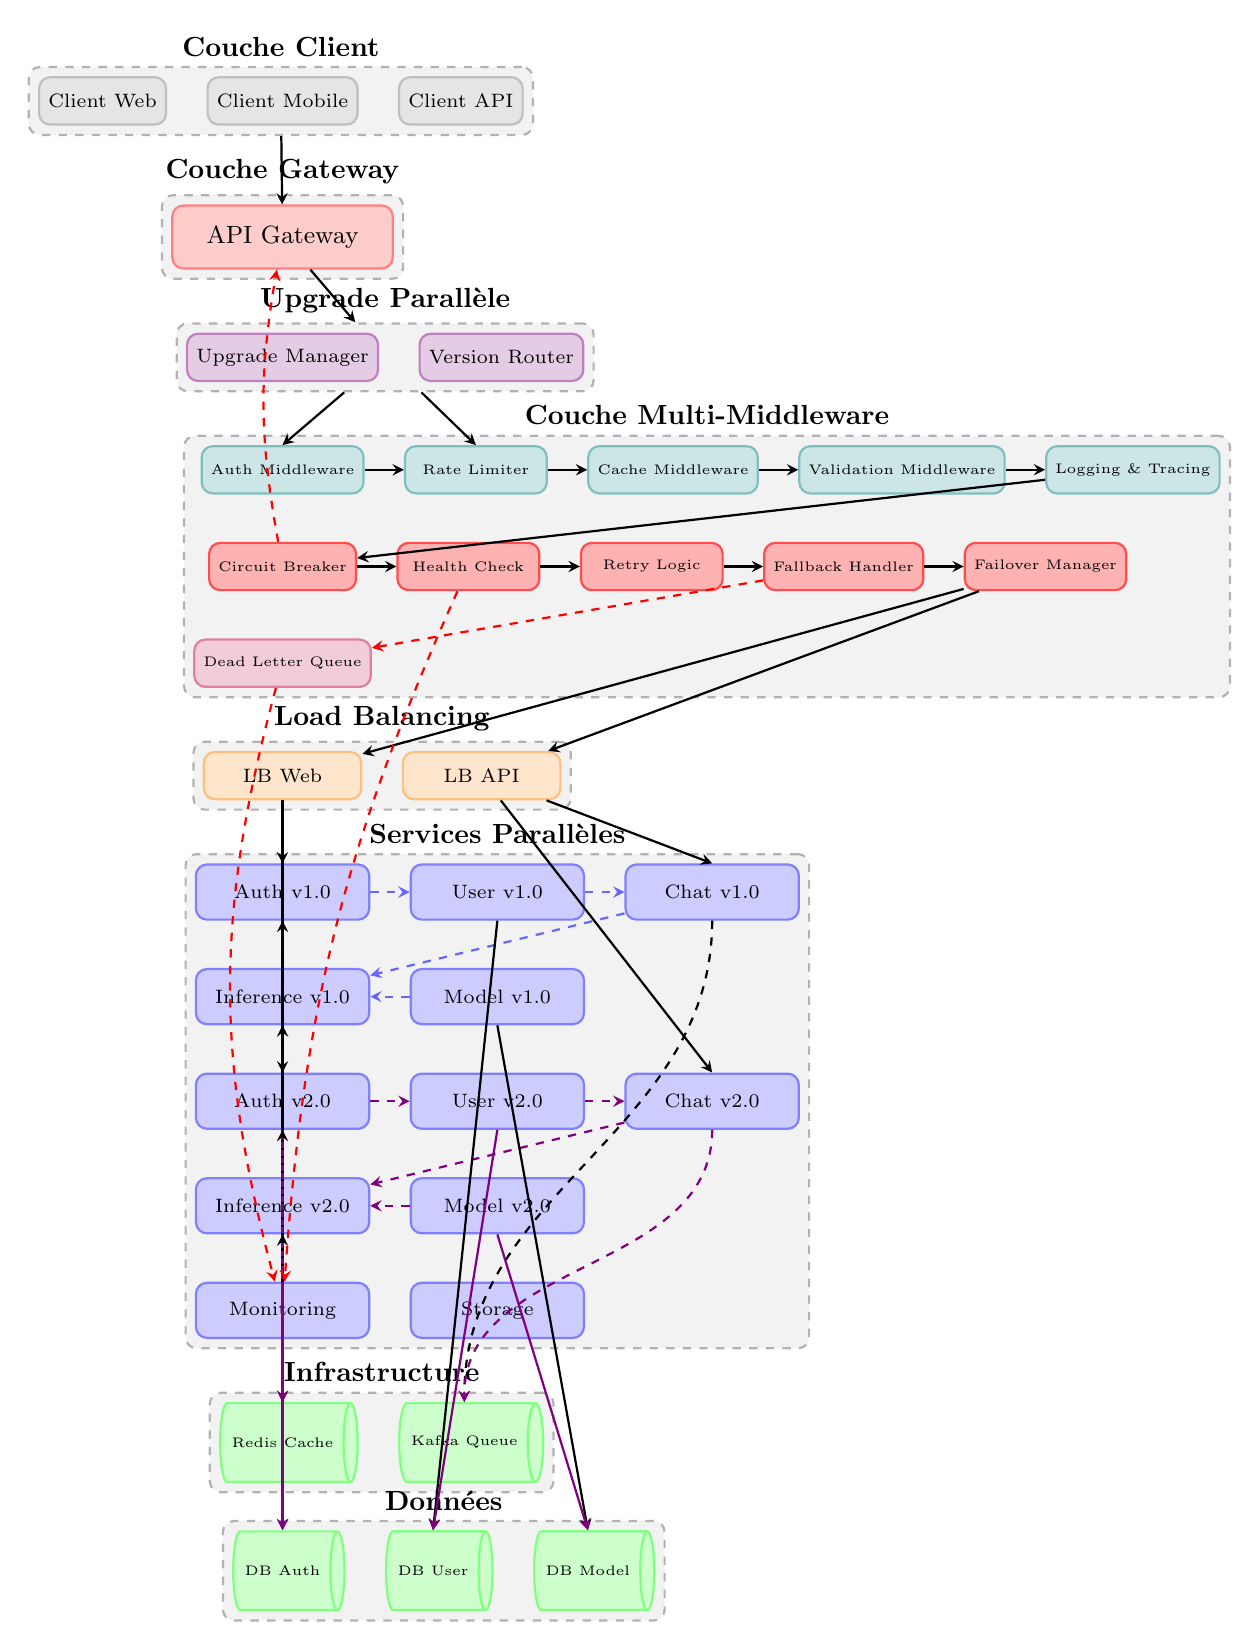
\begin{tikzpicture}[
    node distance=0.7cm and 0.5cm,
    service/.style={rectangle, draw=blue!50, fill=blue!20, thick, minimum width=2.2cm, minimum height=0.7cm, text centered, rounded corners, font=\scriptsize},
    database/.style={cylinder, draw=green!50, fill=green!20, thick, aspect=0.5, minimum height=0.8cm, minimum width=1cm, font=\tiny},
    gateway/.style={rectangle, draw=red!50, fill=red!20, thick, minimum width=2.8cm, minimum height=0.8cm, rounded corners, font=\small},
    loadbalancer/.style={rectangle, draw=orange!50, fill=orange!20, thick, minimum width=2cm, minimum height=0.6cm, rounded corners, font=\scriptsize},
    middleware/.style={rectangle, draw=teal!50, fill=teal!20, thick, minimum width=1.8cm, minimum height=0.6cm, rounded corners, font=\tiny},
    fallback/.style={rectangle, draw=red!70, fill=red!30, thick, minimum width=1.8cm, minimum height=0.6cm, rounded corners, font=\tiny},
    upgrade/.style={rectangle, draw=violet!50, fill=violet!20, thick, minimum width=2cm, minimum height=0.6cm, rounded corners, font=\scriptsize},
    queue/.style={rectangle, draw=purple!50, fill=purple!20, thick, minimum width=1.8cm, minimum height=0.6cm, rounded corners, font=\tiny},
    client/.style={rectangle, draw=gray!50, fill=gray!20, thick, minimum width=1.5cm, minimum height=0.6cm, rounded corners, font=\scriptsize},
    layer/.style={rectangle, draw=black!30, dashed, thick, fill=black!5, rounded corners},
    arrow/.style={->, >=stealth, thick},
    redarrow/.style={->, >=stealth, thick, red, dashed},
    upgradearrow/.style={->, >=stealth, thick, violet}
]

% ============ COUCHE CLIENT ============
\node[client] (web-client) {Client Web};
\node[client, right=of web-client] (mobile-client) {Client Mobile};
\node[client, right=of mobile-client] (api-client) {Client API};

\begin{scope}[on background layer]
\node[layer, fit=(web-client)(mobile-client)(api-client), label=above:\textbf{Couche Client}] (client-layer) {};
\end{scope}

% ============ COUCHE GATEWAY ============
\node[gateway, below=1cm of mobile-client] (api-gateway) {API Gateway};

\begin{scope}[on background layer]
\node[layer, fit=(api-gateway), label=above:\textbf{Couche Gateway}] (gateway-layer) {};
\end{scope}

% ============ COUCHE UPGRADE PARALLELE ============
\node[upgrade, below=0.8cm of api-gateway] (upgrade-manager) {Upgrade Manager};
\node[upgrade, right=of upgrade-manager] (version-router) {Version Router};

\begin{scope}[on background layer]
\node[layer, fit=(upgrade-manager)(version-router), label=above:\textbf{Upgrade Parallèle}] (upgrade-layer) {};
\end{scope}

% ============ COUCHE MULTI-MIDDLEWARE COMPLETE ============
% Ligne 1: Middlewares de base
\node[middleware, below=0.8cm of upgrade-manager] (auth-middleware) {Auth Middleware};
\node[middleware, right=of auth-middleware] (rate-limiter) {Rate Limiter};
\node[middleware, right=of rate-limiter] (cache-middleware) {Cache Middleware};
\node[middleware, right=of cache-middleware] (validation-middleware) {Validation Middleware};
\node[middleware, right=of validation-middleware] (logging-tracing) {Logging \& Tracing};

% Ligne 2: Middlewares de résilience
\node[fallback, below=0.6cm of auth-middleware] (circuit-breaker) {Circuit Breaker};
\node[fallback, right=of circuit-breaker] (health-check) {Health Check};
\node[fallback, right=of health-check] (retry-logic) {Retry Logic};
\node[fallback, right=of retry-logic] (fallback-handler) {Fallback Handler};
\node[fallback, right=of fallback-handler] (failover-manager) {Failover Manager};

% Ligne 3: Queue pour les échecs
\node[queue, below=0.6cm of circuit-breaker] (dlq) {Dead Letter Queue};

\begin{scope}[on background layer]
\node[layer, fit=(auth-middleware)(rate-limiter)(cache-middleware)(validation-middleware)(logging-tracing)(circuit-breaker)(health-check)(retry-logic)(fallback-handler)(failover-manager)(dlq), 
      label=above:\textbf{Couche Multi-Middleware}] (middleware-layer) {};
\end{scope}

% ============ COUCHE LOAD BALANCING ============
\node[loadbalancer, below=0.8cm of dlq] (lb-web) {LB Web};
\node[loadbalancer, right=of lb-web] (lb-api) {LB API};

\begin{scope}[on background layer]
\node[layer, fit=(lb-web)(lb-api), label=above:\textbf{Load Balancing}] (lb-layer) {};
\end{scope}

% ============ COUCHE SERVICES PARALLELES ============
% Services version 1.0
\node[service, below=0.8cm of lb-web] (auth-v1) {Auth v1.0};
\node[service, right=of auth-v1] (user-v1) {User v1.0};
\node[service, right=of user-v1] (chat-v1) {Chat v1.0};

\node[service, below=0.6cm of auth-v1] (inference-v1) {Inference v1.0};
\node[service, right=of inference-v1] (model-v1) {Model v1.0};

% Services version 2.0
\node[service, below=0.6cm of inference-v1] (auth-v2) {Auth v2.0};
\node[service, right=of auth-v2] (user-v2) {User v2.0};
\node[service, right=of user-v2] (chat-v2) {Chat v2.0};

\node[service, below=0.6cm of auth-v2] (inference-v2) {Inference v2.0};
\node[service, right=of inference-v2] (model-v2) {Model v2.0};

% Services support
\node[service, below=0.6cm of inference-v2] (monitoring) {Monitoring};
\node[service, right=of monitoring] (storage) {Storage};

\begin{scope}[on background layer]
\node[layer, fit=(auth-v1)(user-v1)(chat-v1)(inference-v1)(model-v1)(auth-v2)(user-v2)(chat-v2)(inference-v2)(model-v2)(monitoring)(storage), 
      label=above:\textbf{Services Parallèles}] (services-layer) {};
\end{scope}

% ============ COUCHE INFRASTRUCTURE ============
\node[database, below=0.8cm of monitoring] (cache) {Redis Cache};
\node[database, right=of cache] (mq) {Kafka Queue};

\begin{scope}[on background layer]
\node[layer, fit=(cache)(mq), label=above:\textbf{Infrastructure}] (infra-layer) {};
\end{scope}

% ============ COUCHE DONNÉES ============
\node[database, below=0.6cm of cache] (db-auth) {DB Auth};
\node[database, right=of db-auth] (db-user) {DB User};
\node[database, right=of db-user] (db-model) {DB Model};

\begin{scope}[on background layer]
\node[layer, fit=(db-auth)(db-user)(db-model), label=above:\textbf{Données}] (data-layer) {};
\end{scope}

% ============ CONNEXIONS SIMPLIFIEES ============
% Client -> Gateway
\draw[arrow] (client-layer) -- (api-gateway);

% Gateway -> Upgrade
\draw[arrow] (api-gateway) -- (upgrade-layer);

% Upgrade -> Middleware (connexions principales)
\draw[arrow] (upgrade-layer) -- (auth-middleware.north);
\draw[arrow] (upgrade-layer) -- (rate-limiter.north);

% Middleware chain (flux principal)
\draw[arrow] (auth-middleware) -- (rate-limiter);
\draw[arrow] (rate-limiter) -- (cache-middleware);
\draw[arrow] (cache-middleware) -- (validation-middleware);
\draw[arrow] (validation-middleware) -- (logging-tracing);
\draw[arrow] (logging-tracing) -- (circuit-breaker);
\draw[arrow] (circuit-breaker) -- (health-check);
\draw[arrow] (health-check) -- (retry-logic);
\draw[arrow] (retry-logic) -- (fallback-handler);
\draw[arrow] (fallback-handler) -- (failover-manager);

% Middleware -> Load Balancing
\draw[arrow] (failover-manager) -- (lb-web);
\draw[arrow] (failover-manager) -- (lb-api);

% Load Balancing -> Services (flèches groupées)
\draw[arrow] (lb-web) -- (auth-v1.north);
\draw[arrow] (lb-web) -- (auth-v2.north);
\draw[arrow] (lb-api) -- (chat-v1.north);
\draw[arrow] (lb-api) -- (chat-v2.north);

% Communication entre services (flèches groupées)
\draw[arrow, dashed, blue!60] (auth-v1) -- (user-v1);
\draw[arrow, dashed, blue!60] (user-v1) -- (chat-v1);
\draw[arrow, dashed, blue!60] (chat-v1) -- (inference-v1);
\draw[arrow, dashed, blue!60] (model-v1) -- (inference-v1);

\draw[upgradearrow, dashed] (auth-v2) -- (user-v2);
\draw[upgradearrow, dashed] (user-v2) -- (chat-v2);
\draw[upgradearrow, dashed] (chat-v2) -- (inference-v2);
\draw[upgradearrow, dashed] (model-v2) -- (inference-v2);

% Services -> Infrastructure
\draw[arrow, dashed] (auth-v1.south) to[out=-90, in=90] (cache.north);
\draw[arrow, dashed] (chat-v1.south) to[out=-90, in=90] (mq.north);
\draw[upgradearrow, dashed] (auth-v2.south) to[out=-90, in=90] (cache.north);
\draw[upgradearrow, dashed] (chat-v2.south) to[out=-90, in=90] (mq.north);

% Services -> Databases
\draw[arrow] (auth-v1.south) -- (db-auth.north);
\draw[arrow] (user-v1.south) -- (db-user.north);
\draw[arrow] (model-v1.south) -- (db-model.north);
\draw[upgradearrow] (auth-v2.south) -- (db-auth.north);
\draw[upgradearrow] (user-v2.south) -- (db-user.north);
\draw[upgradearrow] (model-v2.south) -- (db-model.north);

% Monitoring connections
\draw[arrow, dotted] (monitoring) -- (auth-v1);
\draw[arrow, dotted] (monitoring) -- (inference-v1);
\draw[arrow, dotted] (monitoring) -- (auth-v2);
\draw[arrow, dotted] (monitoring) -- (inference-v2);

% Circuit breaker fallback vers Gateway
\draw[redarrow] (circuit-breaker) to[bend left=10] (api-gateway);

% Health check vers Monitoring
\draw[redarrow] (health-check) to[bend right=10] (monitoring);

% Fallback handler vers DLQ
\draw[redarrow] (fallback-handler) -- (dlq);

% DLQ vers Monitoring pour analyse
\draw[redarrow, dashed] (dlq) to[bend right=15] (monitoring);

\end{tikzpicture}
\caption{Architecture Microservices Parallèle et Multi-Middleware de Deepseek}
\label{fig:upgrade-architecture}
\end{figure}

\end{document}